\documentclass{standalone}
\usepackage{amsmath,amssymb}
\usepackage[dvipsnames]{xcolor}
\usepackage{tikz} 
\usetikzlibrary{arrows, decorations.markings,decorations.pathreplacing,angles,quotes}
\usepackage{microtype}
\usepackage{fourier}

\definecolor{np}{rgb}{0.5, 0, 0.5}
\definecolor{nb}{RGB}{31,119,180}
\definecolor{no}{RGB}{255,127,14}
\definecolor{ng}{rgb}{0,0.5,0}

%include other needed packages here   
\begin{document}

\begin{tikzpicture}
% include your tikz code here
    		\node[anchor=south west,inner sep=0] (Bild) at (0,0) {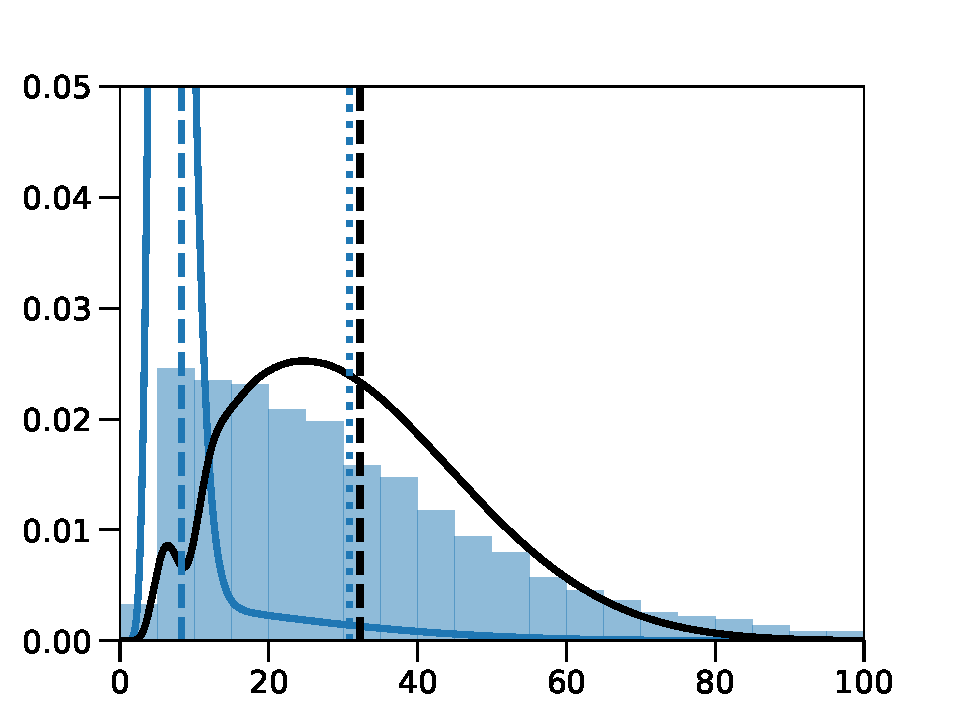
\includegraphics[scale=0.39]{figS5a_blank.pdf}};
   		\begin{scope}[x=(Bild.south east),y=(Bild.north west)]
        	\draw (0.55,-0.035) node {first sampling time};
        	\draw (-0.01,0.5) node [rotate=90] {probability density};
        	%\draw (0.7,0.65) node {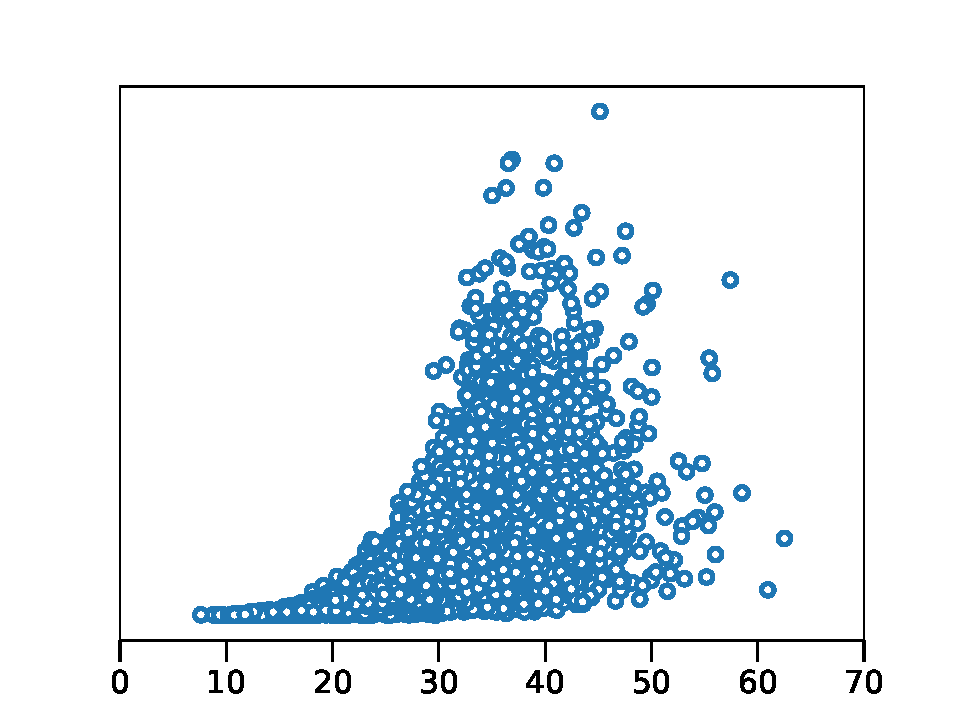
\includegraphics[scale=0.15]{fig4a_scatter.pdf}};
        	%\draw (0.7,0.45) node {\tiny time};
        	%\draw (0.535,0.65) node[rotate = 90] {\tiny size};
        	
        	\draw[color = nb, very thick] (0.575,0.78) -- node[right=6pt] {\color{black} \small Eq. (9)} (0.625,0.78);
        	\draw[color = black, very thick] (0.575,0.7) -- (0.625,0.7);
        	\draw (0.625,0.72) node[right=2pt] {\tiny McKendrick-};
        	\draw (0.625,0.68) node[right=2pt] {\tiny von Foerster approx.};
        	\draw[color = nb, very thick,dashed] (0.575,0.62) -- (0.625,0.62);
        	\draw[color = black, very thick,dashed] (0.575,0.58) -- (0.625,0.58);
        	\draw (0.6,0.62) node[right=6pt] {\color{black} \small analytical};
        	\draw (0.6,0.58) node[right=6pt] {\small mean};
        	\draw[color = nb, very thick,dotted] (0.575,0.485) -- (0.625,0.485);
        	\draw (0.6,0.51) node[right=6pt] {\color{black} \small simulation};
        	\draw (0.6,0.46) node[right=6pt] {\small mean};
    		\end{scope}
\end{tikzpicture}

\end{document}